\chapter{Background}  \label{sec:background}

This chapter provides an overview of the key concepts relevant to this thesis, including \ac{pprl}, various encoding techniques used in secure linkage and existing attacks on encodings and \ac{pprl} schemes.
\ac{pprl} enables different organizations to link records belonging to the same individual across datasets while preserving privacy, making it a crucial tool.
However, the security of such methods can depend on the encoding techniques used to transform sensitive data into a more privacy-preserving format \cite{vidanage2020graph}.

To understand the vulnerabilities of \ac{pprl} systems, we examine three key encoding techniques: \ac{bf}, \ac{tmh}, and \ac{tsh}, each offering different trade-offs between efficiency, privacy, and robustness against attacks.
While these methods aim to prevent direct access to plaintext identifiers, they remain susceptible to adversarial techniques designed to infer or reconstruct the original data \cite{vidanage2020graph,schaefer2024}.

One such adversarial approach is the \ac{gma}, which leverages structural similarities between encoded and non-encoded datasets to re-identify individuals.
Although \ac{gma}s are good in reconstructing intersections of datasets, they are limited to the intersection of the two datasets.
To extend \ac{gma}s beyond known intersections, we explore \ac{ann}s, which can learn complex patterns in encoded data and increase identification rates \cite{schaefer2024,vidanage2020graph}.

By integrating these concepts, this chapter establishes the necessary foundation for understanding the \ac{dea} introduced later in this thesis, demonstrating how machine learning techniques can be employed to bypass existing privacy-preserving mechanisms.

\section{Overview of \ac{pprl} }\label{sec:pprl_overview}

\ac{pprl} enables the linkage of records from different databases that refer to the same individual while trying to preserve privacy.
Traditional record linkage relies on unique identifiers, but these are often unavailable or inconsistent due to variations in formatting, spelling or missing data in a distributed environment.
Linking records directly on plaintext data poses significant privacy risks.
To mitigate these risks and prevent further threats to individuals, regulations such as the European Union's \ac{gdpr} have been established to govern the handling of \ac{pii} \cite{schaefer2024,vidanage2020graph}.

To enable record linkage using \ac{pii} while trying to preserve privacy, \ac{pprl} employs similarity-preserving encoding on quasi-identifiers, allowing linkage to be performed on encoded representations rather than raw data.
This approach protects identities while still facilitating record matching based on encoded similarities and probabilistic approaches.
But this also causes the security of \ac{pprl} schemes to be dependent on the encoding techniques used \cite{schaefer2024,vidanage2020graph}.


Broadly, \ac{pprl} methods fall into two categories: perturbation based techniques and \ac{smc} based techniques.
\ac{smc}-based techniques provide strong security guarantees and high accuracy but suffer from computational and communication overheads.
Conversely, perturbation-based techniques balance linkage quality, scalability, and privacy protection, making them more practical for real-world applications \cite{vidanage2020graph}.

As seen in Figure~\ref{fig:pprloverview} a typical \ac{pprl} system involves three main parties working together in four steps to enable the linkage while maintaining privacy.
First data owners, who are responsible for maintaining their respective databases, \(D\) and \(D'\), encode the quasi-identifiers by agreeing on an encoding scheme with the corresponding parameters before then as a second step sharing their respective data sets with the linkage unit.
The linkage unit, a trusted entity, performs the actual record linkage using only the encoded representations, without access to the original identifiers.
Once the linkage is completed, the linkage unit assigns unique pseudonyms to the successfully linked records and returns the pseudonymized dataset as a third step to the data owners.
The data owners then replace the linkage data with these pseudonyms before sending the dataset in the fourth and final step to the receipient requesting the data.
In the case of a research project this could be an data analyst.
The data analyst can merge the records based on the identifiers and proceed with further research and analysis, all while minimizing the risk of re-identification and protecting individual privacy \cite{schaefer2024}.

\begin{figure}[H]
  \centering
  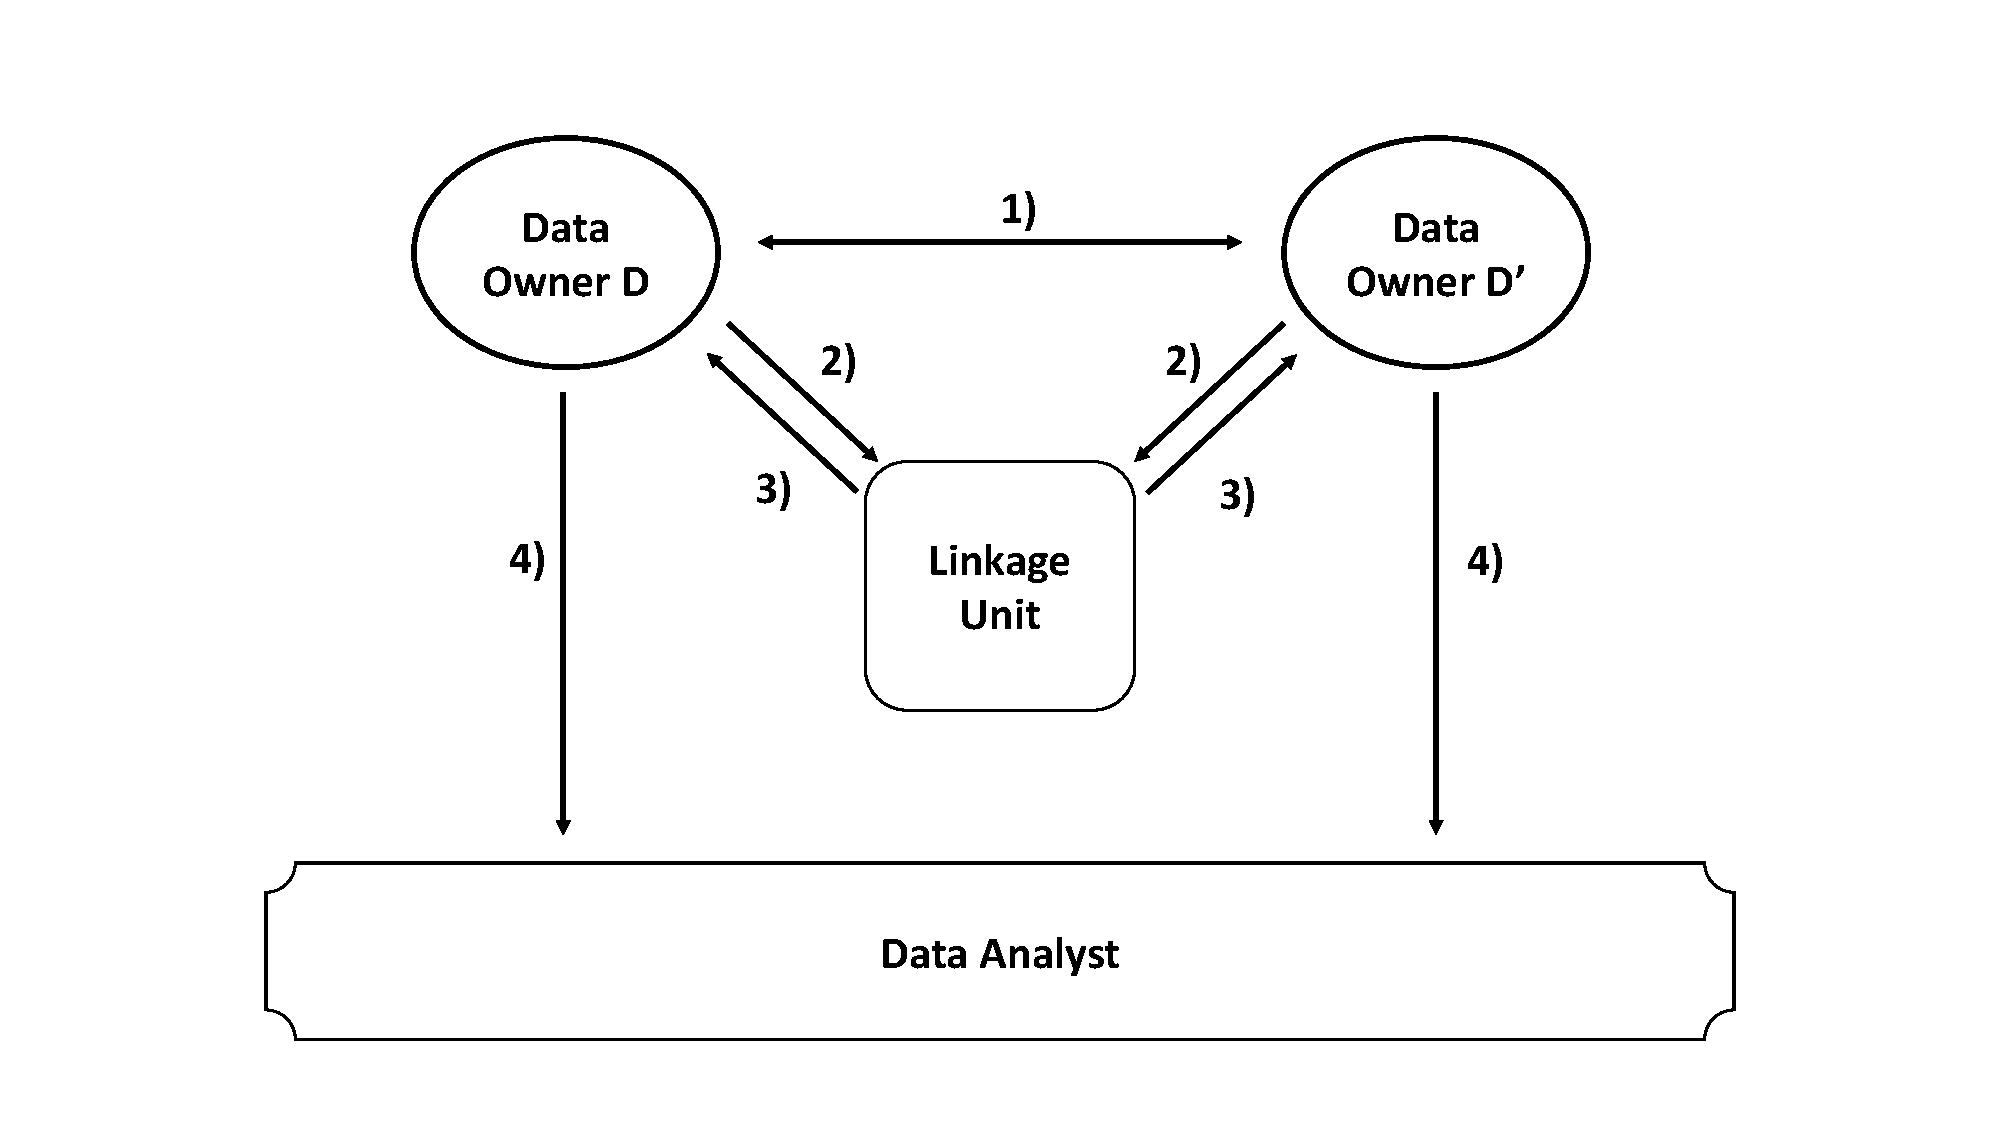
\includegraphics[width=0.66\textwidth, page=1]{img/visualization.pdf}
  \caption{Overview of the \ac{pprl} process.}
  \label{fig:pprloverview}
\end{figure}

Based on this scheme, each database record can therefore during the linkage process be represented as $r = (\lambda,  \sigma)$, where $\lambda$ denotes the linkage data which are encoded quasi-identifiers such as names and birthdates and $\sigma$ refers to the remaining microdata like in a health care scenario patient information \cite{schaefer2024}.

Linkage in \ac{pprl} is performed probabilistically, meaning that two records, \(r\) and \(r'\), are considered linked if their similarity score on \(sim(\lambda_r, \lambda_{r'})\) exceeds a predefined threshold.
The choice of threshold plays a crucial role in balancing the quality of the linkage.
Lower thresholds tolerate more variation and matches between records but increase the likelihood of false positives, while higher thresholds reduce false positives but may miss legitimate matches.
Thus, selecting the optimal threshold is a trade-off that requires careful consideration of the specific goals and constraints of the linkage process \cite{schaefer2024}.

A robust \ac{pprl} scheme must satisfy several important criteria to ensure effective and secure linkage.
First, a similarity function, \(sim(\lambda_r, \lambda_{r'})\), must exist to determine if two records belong to the same entity based on a predefined threshold.
Second, an encoding scheme \(enc(\lambda)\)  must be applied to \(\lambda\) in such a way that the linkage unit cannot reconstruct the original data.
Finally, a function \(sim(enc(\lambda_r), enc(\lambda_{r'}))\) must be available that allows similarity computations on encoded data which preserved similarty properties.
These requirements ensure both the privacy and the effectiveness of the record linkage process \cite{schaefer2024}.

One common approach for measuring similarity for two quasi identifiers and enabling probabilistic matching on quasi identifieres is using n-grams.
Here, string values are divided into overlapping substrings of length $n$ using a sliding window approach \cite{schaefer2024}.
For example, for the string ``encoding'' with $n=2$, the n-grams are:
$$ \{\text{en}, \text{nc}, \text{co}, \text{od}, \text{di}, \text{in}, \text{ng} \} $$

The similarity of two sets of n-grams can then be computed using metrics such as the Dice Coefficient where X and Y denotes two sets which are in the case of \ac{pprl} the n-grams for two different pseudo identifiers \cite{schaefer2024}.
  $$ Dice(X, Y) = \frac{2 \times |X \cap Y|}{|X| + |Y|} $$
The Jaccard Similarity can be used in a similar way \cite{schaefer2024}.
  $$ Jaccard(X, Y) = \frac{|X \cap Y|}{|X \cup Y|} $$

\ac{pprl} has been successfully applied in various domains, demonstrating its practical importance in securely linking records across institutions while trying to preserve privacy.
Notable applications include the Social Investment Data Resources, the Lumos Initiative, the Swiss National Cohort, and the Gemeinsamer Bundesausschuss.
These implementations highlight the versatility of \ac{pprl} in diverse contexts, where privacy protection is essential while enabling effective data linkage for research and analysis \cite{schaefer2024}.



\section{Key Encoding Techniques} \label{sec:key-encodings}

In the context of \ac{pprl}, three primary encoding techniques have emerged: \ac{bf}, \ac{tmh} and \ac{tsh}.
These encoding methods are essential for transforming sets of quasi-identifiers into representations that preserve similarity information while trying to maintain privacy \cite{schaefer2024,vidanage2020graph, schnell2009privacy}.

\ac{pprl} typically involves encoding sets of quasi-identifiers before linkage.
A set in this context is generally a collection of n-grams, which are substrings of length $n$ extracted from one or multiple attributes using a sliding window approach.
Since input data varies in length, all encoding techniques in \ac{pprl} must take arbitrarily long inputs (sets of n-grams) and produce encoded outputs.
This ensures that similarity computations can be efficiently performed on encoded data by the linkage unit without accessing the raw identifiers \cite{vidanage2020graph,schaefer2024}.

Before linkage, data owners must agree on the encoding scheme and share necessary cryptographic secrets to facilitate secure comparison.
Among the available techniques, \ac{bf}s are the most widely used approach for record linkage \cite{schaefer2024}.

\subsection{\ac{bf}} \label{sec:bf}

\ac{bf}s were originally developed for efficient membership testing in set structures without requiring direct access to the sets themselves \cite{bloom1970space}.
Due to their ability to efficiently compute set similarities in a privacy-preserving manner, they have been widely adopted in \ac{pprl} applications \cite{schaefer2024,vidanage2020graph,schnell2009privacy}.

A \ac{bf} $b \in \{0,1\}^l$ is a bit vector of length $l$.
It uses $k \geq 1$ independent hash functions $H = \{h_1, h_2, ..., h_k\}$, where each function maps an arbitrary input to a position in the filter \cite{schaefer2024,schnell2009privacy}:
\begin{equation}
  h_i: \{0,1\}^* \to \{1, ..., l\}, \quad \forall i \in \{1, ..., k\}
\end{equation}
Initially, the \ac{bf} is set to all zeros.
Each element $s \in S$ is hashed with every function $h_i$, and the corresponding bit positions in the filter are set to 1 \cite{schaefer2024,schnell2009privacy}:
\begin{equation}
  \forall s \in S, \forall h_i \in H, \quad b[h_i(s)] = 1
\end{equation}

An Example for this can be seen in Figure~\ref{fig:bfexample} where the set of 2-grams for the word ''encoding'' is encoded using a \ac{bf} with $k = 2$ hash functions. As can be seen, the 2-grams are hashed using the two hash functions and the corresponding bits are set to 1 in the \ac{bf}.

\begin{figure}[H]
  \centering
  \includegraphics[width=0.66\textwidth, page=5]{img/visualization.pdf}
  \caption{Example \ac{bf} for $k = 2$ hash functions on the set of 2-grams for ''encoding''.}
  \label{fig:bfexample}
\end{figure}

Since \ac{bf}s are binary vectors, the similarity between two \ac{bf}s, \(b_1\) and \(b_2\), is computed based on the overlapping 1-bits based on their position.
The Dice Coefficient is commonly used for this purpose \cite{schaefer2024}, providing a measure of similarity by comparing the overlap of 1-bits in the two binary vectors.
Therefore encodings using \ac{bf} encoding allows for efficient computation of similarity between two sets which is benefical for \ac{pprl} systems.
\begin{equation}
  \text{Dice}(b_1, b_2) = \frac{2 \cdot |b_1 \cap b_2|}{|b_1| + |b_2|}
\end{equation}

Because the sets in a \ac{pprl} systems consists of n-grams, a deterministic relationship between the n-grams present in the quasi-identifier $\lambda$ and the set bits in the \ac{bf} is created.
However, due to the finite length of \ac{bf}s, collisions occur where different n-grams map to the same bit position (see Figure~\ref{fig:bfexample}).
While this can cause incorrect linkages, it also enhances privacy by distorting frequency distributions \cite{vidanage2020graph,schaefer2024}.

Three primary approaches exist for applying \ac{bf}s to sensitive data.
The first approach, Attribute-Level \ac{bf}s, encodes each attribute, such as first name or last name, into a separate \ac{bf}, enabling multiple similarity computations.
However, Attribute-Level \ac{bf}s are more vulnerable to frequency-based privacy attacks as they lower the collisions which would occur using only one \ac{bf}.
The second approach, Cryptographic Long-Term Key Encoding, merges multiple attributes into a single \ac{bf}, reducing vulnerability to frequency attacks but remaining susceptible to pattern-mining-based attacks.
Finally, Record-Level \ac{bf}s employ a weighted bit sampling technique to minimize frequency information, enhancing privacy protection while maintaining high linkage quality.
Each of these approaches balances privacy concerns with the need for accurate and effective record linkage \cite{vidanage2020graph}.

Several privacy-enhancing methods have been proposed to mitigate frequency attacks in \ac{bf}s.
These techniques introduce a trade-off between privacy and linkage quality.
One such method is balancing, which ensures an equal number of 1-bits across \ac{bf}s, thereby reducing the likelihood of frequency-based attacks.
Another approach is salting, which randomizes bit positions to prevent direct inference from the encoded quasi-identifiers.
Additionally, XOR folding is used to reduce the \ac{bf} length while maintaining the bit-wise dependencies necessary for effective linkage.
These methods aim to strengthen privacy while retaining the accuracy of the linkage process \cite{vidanage2020graph,schaefer2024}.

A major improvement was introduced by Armknecht et al. \cite{armknecht2023strengthening}, who proposed a diffusion layer for \ac{bf} encodings.
This method generates \ac{eld}, where each bit is computed as the XOR sum of multiple \ac{bf} bits.
The indices for XOR computations are randomly chosen and secretly shared among data owners \cite{armknecht2023strengthening}.

By applying diffusion, the deterministic relationship between 1-bits in the \ac{eld} and the original n-grams is broken, improving privacy while still enabling approximate matching \cite{armknecht2023strengthening}.

\ac{bf}s remain a core technique in \ac{pprl} due to their efficiency and scalability.
However, their vulnerability to frequency attacks has led to improvements such as Record-Level \ac{bf}s and diffusion layers, which enhance privacy at the cost of increased computational complexity \cite{schaefer2024, vidanage2020graph,armknecht2023strengthening}.


\subsection{\ac{tmh}} \label{sec:tmh}

\ac{tmh} is a variation of MinHash initially introduced for efficient estimation of set similarities and later adapted for privacy-preserving probabilistic record linkage.
MinHash itself was first proposed in the context of document resemblance and containment estimation.
\ac{tmh} extends MinHash by employing tabulation-based hashing, which enhances its security compared to \ac{bf}s \cite{vidanage2020graph,broder1997resemblance}.

MinHash aims to approximate the Jaccard similarity between two sets, \(S\) and \(S'\).
The fundamental idea is to represent both sets as sequences of randomly ordered elements and apply multiple rounds of random permutations \(\pi\) to shuffle them.
After each round, the first elements of both sequences are compared.
The larger the intersection between \(S\) and \(S'\), the higher the probability that the first elements will match.
An example for this can be seen in Figure~\ref{fig:minhashexample} where the sets are permutated twice and the first element is compared for each new set.
The final Jaccard similarity estimate is computed based on the number of collisions achieved during permutation, in the example is one collision for two permutations \cite{schaefer2024,broder1997resemblance,vidanage2020graph}.

\begin{figure}[H]
  \centering
  \includegraphics[width=0.66\textwidth, page=6]{img/visualization.pdf}
  \caption{Example computing approximate Jaccard similarity using MinHash with \(\pi = 2\) permutations.}
  \label{fig:minhashexample}
\end{figure}

Instead of explicitly computing these permutations, MinHash simulates them by applying a suitable hash function to the elements of a set and selecting the smallest hash value as the representative signature.
This is equivalent to sorting set elements by their hash values and returning the first element \cite{schaefer2024}.

Tabulation-based hashing is a technique used in \ac{tmh} that provides efficient and high-quality hash functions by leveraging precomputed lookup tables.
This method operates as follows \cite{vidanage2020graph}:

The process begins with the \textbf{initialization} of \(l\) sets of lookup tables, each containing \(c\) tables.
Each table holds randomly generated bit strings for keys of length \(k\), with a key space of \(2^k\).
During the \textbf{hashing process}, each element in \(S\) is hashed using a one-way hash function, producing a fixed-length binary value.
This binary value is then split into \(c\) sub-keys, each of length \(k\).
Each sub-key is used as an index to retrieve a random bit string from the corresponding lookup table, and the retrieved \(c\) bit strings are XORed together to produce a single output bit string.
In the \textbf{MinHash signature generation} phase, this process is repeated for each of the \(l\) lookup table sets, and the minimum value among all generated bit strings is selected as the MinHash signature \cite{schaefer2024,vidanage2020graph}.

An example for this can be seen in Figure~\ref{fig:tabminhashexample} where the first element of the set is hashed using the first lookup table and the fourth hash function.
The key is split into \(c = 4\) sub-keys of length \(k = 2\) and used to retrieve the corresponding bit strings from the lookup table.
The retrieved bit strings are then XORed together to produce the final value for the first element.

\begin{figure}[H]
  \centering
  \includegraphics[width=0.66\textwidth, page=7]{img/visualization.pdf}
  \caption{Simplified \ac{tmh} hasing step for the first lookup table, fourth hash function on the first set element.}
  \label{fig:tabminhashexample}
\end{figure}


To further enhance privacy, \ac{tmh} employs a 1-bit hashing mechanism, where only the least significant bit of each MinHash signature is retained.
These $l$ bits are then concatenated to form the final bit array used as an encoded representation \cite{schaefer2024}.

The main advantage of \ac{tmh} over \ac{bf}s is its improved resistance to frequency-based attacks due to the complexity introduced by tabulation-based hashing.
However, this security enhancement comes at a cost.
It leads to higher computational overhead, as the need to generate and access multiple lookup tables increases processing time.
Additionally, there is increased memory consumption because storing large precomputed tables requires additional space.
These trade-offs must be considered when choosing between \ac{tmh} and other privacy-preserving techniques \cite{schaefer2024,vidanage2020graph}.
Despite these trade-offs, \ac{tmh} remains an attractive alternative for \ac{pprl} due to its robustness against adversarial attacks.

Similar to \ac{bf}s, \ac{tmh} encodes each record as a bit vector of length $l$.
Given two \ac{tmh}-encoded bit vectors, their similarity can be estimated using a modified Jaccard coefficient, adapted to account for artificial bit collisions caused by truncation to the least significant bit.
The Jaccard coefficient can also be converted into the Dice coefficient for improved comparability with \ac{bf}-based methods \cite{vidanage2020graph,schaefer2024}.

Overall, \ac{tmh} provides a more secure encoding alternative to \ac{bf}s in \ac{pprl}, though at the expense of increased computational and memory requirements \cite{schaefer2024, vidanage2020graph}.


\subsection{\ac{tsh}} \label{sec:tsh}

\ac{tsh} is the most recent encoding scheme proposed for \ac{pprl}, introduced in 2020 \cite{ranbaduge2020secure}.
\ac{tsh} was designed to address both the privacy vulnerabilities of \ac{bf}s and the computational complexity of \ac{tmh} while maintaining accuracy in similarity calculations.
Similar to other encoding techniques, \ac{tsh} requires the input to be split into a set of n-grams $S$ prior to encoding \cite{ranbaduge2020secure}.

As a result of \ac{tsh} encoding, each record from a sensitive database is represented by a set of integers, which can be directly used to compute Jaccard similarity.
\ac{tsh} employs two distinct hashing steps.
In the first hashing step, the input set is converted into a bit matrix representation.
In the second hashing step, the bit matrix columns are mapped into integers, enabling efficient comparison.
This two-step process allows \ac{tsh} to represent sensitive data in a way that facilitates effective similarity computation while preserving privacy \cite{schaefer2024}.
These steps provide accurate Jaccard similarity calculations while improving privacy protection compared to traditional \ac{bf}-based encodings \cite{ranbaduge2020secure}.

In the first step of the \ac{tsh} process, elements of the n-gram set \(S\) are hashed into \(k\) independent \ac{bf}s \(b_i\) of length \(l\), meaning each hash function results in a corresponding bit vector.
This generates a \(k \times l\) matrix, where each row corresponds to a \ac{bf} created using a unique hash function, and each column represents the bitwise state across all \ac{bf}s for a given position.
In the second step, after constructing the bit matrix, \ac{tsh} computes column-wise hashes to convert the bit vectors into integer representations .
Each column vector is treated as an input for a hash function, and all-zero columns are skipped to prevent distortion in similarity calculations since they do not encode any n-grams.
To enhance security and avoid hash collisions between columns with identical bit patterns, a salt value and the column index are concatenated before hashing \cite{ranbaduge2020secure}.

The final integer representation for each column $i$ for $1 \leq i \leq l$. is computed as \cite{schaefer2024, ranbaduge2020secure}:
\begin{equation}
    H(salt, i, b_{1i}, b_{2i}, ..., b_{ki})
\end{equation}

The output of the second hashing step is a set of integers, allowing similarity computations using the Dice coefficient rather than directly computing bitwise similarity.
Since the encoded data consists of sets, Jaccard similarity can also be computed similarly to MinHash-based encodings \cite{ranbaduge2020secure}.

\begin{figure}[H]
  \centering
  \includegraphics[width=0.66\textwidth, page=8]{img/visualization.pdf}
  \caption{\ac{tsh} example for for two input values ''peter'' and ''pete'' \cite{ranbaduge2020secure}.}
  \label{fig:tshexample}
\end{figure}

An illustrative example is provided in Figure~\ref{fig:tshexample}, where the set of 2-grams for the words ``\textit{peter}'' and ``\textit{pete}'' is encoded using \ac{tsh} with $k = 4$ hash functions and a Bloom filter length of $l = 8$.
In the first hashing step, each 2-gram is processed using the $k$ hash functions, resulting in a $4 \times 8$ bit matrix.
Each row of this matrix corresponds to a Bloom filter generated with a distinct hash function, encoding the presence of 2-grams across the $l$ bit positions.

In the second hashing step, the columns of the bit matrix are transformed into integer values.
This is achieved by applying an additional hash function that incorporates both a salt value and the column index, effectively compressing the binary representation into a fixed-length integer vector.
The final output is a set of integers representing the encoded word, which can subsequently be used to compute similarity scores between different words~\cite{ranbaduge2020secure}.

To improve efficiency, \ac{tsh} can be implemented using a \ac{prng} instead of cryptographic hash functions.
The \ac{prng} is seeded with the value to be hashed before generating random numbers, ensuring that the sequence of generated values depends deterministically on the input \cite{ranbaduge2020secure}.

By combining efficient bit vector representations with integer-based similarity computations, \ac{tsh} offers a balance between privacy, security, and computational efficiency, making it a promising alternative to existing \ac{pprl} encoding schemes \cite{vidanage2020graph, ranbaduge2020secure}.

\section{\ac{gma}} \label{sec:gma}

\ac{gma}s  were introduced by Vidanage et al. \cite{vidanage2020graph} and represent the most significant threat to \ac{pprl} due to their universal applicability.
Unlike traditional cryptanalytic attacks, \ac{gma}s exploit the fundamental properties of non-interactive \ac{pprl} to compromise the security of all schemes relying on similarity-preserving encoding \cite{schaefer2024}.


Non-interactive \ac{pprl} refers to linkage schemes where data owners independently encode their data and share it with a linkage unit.
The linkage unit then performs record matching solely based on the encoded data, without requiring further interaction with the data owners during the linkage process.
This approach minimizes communication overhead and computational complexity, as no iterative exchanges between parties are necessary.
In contrast, interactive PPRL methods involve multiple rounds of communication between data owners and the linkage unit to refine matching results or improve accuracy \cite{kum2014privacy}.

In \ac{pprl}, encoded records are linked based on similarity computations.
Since these similarities serve as identifiers, an attacker with access to both encoded and plaintext data can leverage them to re-identify individuals.
The latest version of the \ac{gma} developed by Schaefer et al. \cite{schaefer2024} overcomes the limitations of the original attack by Vidanage et al. \cite{vidanage2020graph} and enhances success rate and robustness, even under limited knowledge scenarios \cite{schaefer2024}.

In the context of a \ac{gma} on a \ac{pprl} system, the attacker is modeled as the linkage unit and is assumed to have minimal prior knowledge.
The attacker does not know any encoding secrets, seeds, or salts used in the system to protect the data.
The only information available to the attacker is that which is inevitably known to the linkage unit during the linkage process.
This assumption ensures that the attacker can only exploit data accessible through normal system operations, adhering to Kerckhoffs's principle \cite{schaefer2024}.

Since the attack does not depend on specific encoding parameters or attribute frequency distributions, it is universally applicable as long as pairwise similarities of encoded data are available \cite{schaefer2024}.

The first step of the attack involves constructing similarity graphs for both the encoded dataset (\(D_{enc}\)) and the plaintext dataset (\(D_{plain}\)).
In these graphs, each node represents an individual record, while edges between nodes are assigned weights based on pairwise similarity computations.
To ensure computational efficiency and focus only on meaningful connections, edges with similarity scores below a predefined threshold are omitted, reducing noise and improving the accuracy of the attack \cite{schaefer2024}.

Since certain encoding properties, such as \ac{bf} length ($l$), are inevitably known to the linkage unit, $D_{plain}$ can be transformed analogously to $D_{enc}$ for effective comparison.
Importantly, this step does not require knowledge of shared secrets, as the primary objective is to replicate the effect of encoding on similarity \cite{schaefer2024}.

To quantify the structural similarity between nodes in \(G_{plain}\) and \(G_{enc}\), node embeddings are computed to transform the graph structure into a numerical representation.
This process begins with graph embedding using the Node2Vec algorithm, which applies a Word2Vec-like approach to learn vector representations of nodes.
During this process, nodes undergo multiple random walks, where each walk simulates a sequence of transitions between connected nodes.
These sequences are then treated as sentences, allowing the model to learn embeddings that capture the local and global structure of the graph.
The behavior of these random walks is controlled by two hyperparameters: \(p\), which determines the likelihood of returning to a previously visited node, and \(q\), which influences the tendency to explore new regions of the graph.
The result is an embedding matrix where each row represents a node as a vector in Euclidean space \cite{schaefer2024}.

Once embeddings are generated, they must be aligned to allow meaningful comparison between the two graphs.
Due to the randomness inherent in embedding generation, direct comparison is not possible.
Instead, an iterative approach is used to solve two subproblems: first, an optimal linear transformation is determined using Procrustes Analysis to align the embeddings, and second, node correspondences are established via the Sinkhorn Algorithm, which minimizes the Wasserstein distance between the distributions of embeddings in both graphs.
To achieve an effective alignment, an unsupervised stochastic optimization scheme alternates between these two steps over \(n\) epochs, gradually refining the transformation and correspondences until convergence \cite{schaefer2024}.

Once the embeddings from the plaintext and encoded datasets are aligned, the reidentification process can begin.
Each embedding in the transformed plaintext space is compared to its counterparts in the encoded space, with similarity measured using cosine similarity.
This metric quantifies how closely two embeddings align in the high-dimensional space, enabling the attacker to identify records in the encoded dataset that most closely resemble those in the plaintext dataset \cite{schaefer2024}.

The final step involves constructing a bipartite graph, where nodes from the plaintext and encoded datasets are linked based on their similarity scores.
To determine the optimal mapping, the Jonker-Volgenant algorithm is applied, ensuring that each node in the smaller dataset is uniquely matched to a corresponding node in the larger dataset.
This algorithm maximizes the total similarity across all matched pairs, effectively revealing the identities of individuals within the encoded dataset \cite{schaefer2024}.

An example of this process is illustrated in Figures~\ref{fig:gmaexampleone} and \ref{fig:gmaexampletwo}, which provide a high-level overview of the \ac{gma} attack applied to a \ac{pprl} approach using \ac{bf} encoding.
Initially, the two data owners agree on an encoding scheme and encode their respective datasets, for this example using Bloom filters.
These encoded datasets are then send to the linkage unit.
The attack begins at this point, leveraging information inherently available to the linkage unit.
Specifically, the linkage unit constructs similarity graphs for both the encoded datasets and an auxiliary plaintext dataset.
By embedding these similarity graphs into a vector space and aligning the embeddings, the attacker can identify re-identifications by comparing embeddings and constructing a bipartite graph that matches entries from the encoded dataset to those in the plaintext auxiliary dataset \cite{schaefer2024}.


\begin{figure}[H]
  \centering
  \includegraphics[width=0.66\textwidth, page=10]{img/visualization.pdf}
  \caption{High-level overview of the \ac{gma} attack process.
  Two data owners encode their datasets and send them to the linkage unit.}
  \label{fig:gmaexampleone}
\end{figure}

\begin{figure}[H]
  \centering
  \includegraphics[width=0.66\textwidth, page=11]{img/visualization.pdf}
  \caption{High-level overview of the \ac{gma} attack process.
  The linkage unit mimics the \ac{bf} encoding for the public dataset and creates for both datasets similartie graphs, embeddings and aligns them to perform bipartite matching.}
  \label{fig:gmaexampletwo}
\end{figure}

The novel \ac{gma} approach by Schaefer et al. \cite{schaefer2024} achieves near-perfect re-identification rates when dataset overlap is 100\%.
Even for low-overlap scenarios (e.g., 5\%), success rates reach 99.9\% for \ac{tsh} \cite{schaefer2024}.
The only encoding scheme resistant to \ac{gma}s is \ac{bf}s with diffusion layers, which disrupts similarity preservation for sufficiently high diffusion values \cite{schaefer2024}.


\section{\ac{ann}} \label{sec:nn}

\ac{ann}s are a class of machine learning models inspired by the structure and function of biological neural systems.
They consist of interconnected layers of artificial neurons that process input data and extract meaningful patterns through iterative learning.
\ac{ann}s have been widely applied in various fields, including image recognition, natural language processing, and classification tasks.
Neural networks are particularly effective for complex tasks because they automatically identify and refine patterns in data through multiple layers of processing, removing the need for manual feature engineering, which can be difficult and time-consuming \cite{dongare2012introduction}.

The structure of an \ac{ann} consists of multiple layers as can be seen in Figure~\ref{fig:annexample}, each serving a distinct role in processing and transforming input data.
The input layer is the first stage of the network, responsible for receiving raw data and forwarding it to subsequent layers.
The number of neurons in this layer corresponds directly to the number of input features, ensuring that all relevant information is passed through the network \cite{dongare2012introduction}.

\begin{figure}[H]
  \centering
  \includegraphics[width=0.66\textwidth, page=16]{img/visualization.pdf}
  \caption{\ac{ann} consisting of multiple input neurons (input layer), hidden layers and output neurons (output layer) \cite{annimage}.}
  \label{fig:annexample}
\end{figure}


Following the input layer are the hidden layers, which perform feature extraction and transformation.
Each neuron in a layer applies a weighted sum operation to its inputs, followed by an activation function that introduces non-linearity, enabling the network to learn complex patterns in the data. Common activation functions include the Rectified Linear Unit (ReLU), Sigmoid, Leaky ReLU, and Exponential Linear Unit (ELU), each offering advantages depending on the specific task \cite{sharma2017activation,russell2016artificial}.

\begin{figure}[H]
  \centering
  \includegraphics[width=0.66\textwidth, page=17]{img/visualization.pdf}
  \caption{Sketch of an single artifical neuron in an \ac{ann} \cite{neuronimage}.}
  \label{fig:neuronexample}
\end{figure}

An example of this process is illustrated in Figure~\ref{fig:neuronexample}, which depicts a single neuron in an \ac{ann}.
The neuron takes multiple inputs, multiplies them by corresponding weights, sums the weighted inputs along with a bias term, and applies an activation function to compute the final output.
Mathematically, this operation is represented as

\begin{equation}
  a = \sigma(z) = \sigma\left(\sum_{i=1}^{n} w_i x_i + b\right)
\end{equation}

where \(a\) is the neuron’s output, \(\sigma\) is the activation function, \(z\) is the weighted sum, \(w_i\) are the weights, \(x_i\) are the inputs, and \(b\) is the bias term \cite{neuronimage}.

The depth and size of the hidden layers determine the network's capacity to model intricate relationships, making them a crucial component of deep learning architectures \cite{dongare2012introduction}.

Finally, the output layer generates the final predictions based on the processed information.
The number of neurons in this layer depends on the nature of the task—whether it is a classification problem, where each neuron represents a class, or a regression task, where a single neuron outputs a continuous value \cite{dongare2012introduction}.

Training an \ac{ann} involves iteratively adjusting its parameters, using a labeled dataset to minimize prediction errors.
The process begins with forward propagation, where input data flows through the network, passing through multiple layers until it reaches the output layer, generating a prediction.
This prediction is then compared to the actual target value, and the discrepancy between the two is quantified using a loss function, which measures the model's performance \cite{russell2016artificial}.

To improve accuracy, the network undergoes backward propagation (backpropagation), where the gradient of the loss with respect to each weight is computed using the chain rule of differentiation.
These gradients indicate how each parameter should be adjusted to reduce the overall error \cite{russell2016artificial}.

An optimizer, such as Stochastic Gradient Descent (SGD) or Adam, updates the weights accordingly by taking small steps in the direction that minimizes the loss.
The training process is repeated over multiple epochs, where the entire dataset is processed multiple times.
To enhance efficiency, the data is often divided into batches, allowing the model to update its weights incrementally rather than processing the entire dataset at once.
Over time, this iterative optimization process enables the network to learn meaningful patterns and improve its predictive performance.
\ac{ann}s can be applied to different classification tasks, depending on whether a data instance belongs to a single category or multiple categories simultaneously \cite{russell2016artificial}.

In traditional single-label or binary classification problems, each instance is assigned to one and only one category from a predefined set of classes.
To achieve this, the network's output layer typically uses a Softmax activation function, which converts the raw output scores into a probability distribution over all possible classes.
The model can be trained using the Cross-Entropy Loss function, which penalizes incorrect classifications by measuring the difference between the predicted probability distribution and the actual class label \cite{russell2016artificial,herrera2016multilabel}.

In contrast, multi-label classification allows an instance to belong to multiple categories at the same time.
Instead of a single categorical output, the network produces independent predictions for each possible label.
The output layer can then as an example apply sigmoid activations for each label, transforming the raw scores into independent probabilities indicating the presence or absence of each class.
Since each label is treated as a separate binary classification problem, Binary Cross-Entropy (BCE) Loss is commonly used to optimize the model, ensuring accurate predictions across multiple labels \cite{russell2016artificial,herrera2016multilabel}.

Different \ac{ann} architectures have been developed to address various problem domains, each optimized for specific types of data and tasks.
Feedforward \ac{ann}s (FNNs) represent the simplest architecture, where data flows in one direction from the input layer to the output layer without forming cycles.
These networks are widely used for basic classification and regression tasks but may struggle with complex patterns that require spatial or sequential dependencies \cite{russell2016artificial,glorot2010understanding}.

For tasks involving image processing, Convolutional \ac{ann}s (CNNs) are commonly used.
CNNs employ convolutional layers that apply filters to input images, allowing the network to capture complex patterns such as edges, textures, and shapes.
This makes them highly effective for applications like object recognition and medical imaging \cite{o2015introduction}.

When dealing with sequential data, Recurrent \ac{ann}s (RNNs) and their advanced variant, Long Short-Term Memory (LSTM) Networks, are particularly useful.
These architectures introduce recurrent connections, enabling them to maintain memory of previous inputs and recognize patterns over time.
This makes them well-suited for natural language processing, speech recognition, and time series forecasting \cite{medsker2001recurrent}.

\subsection{PyTorch for Training \ac{ann}} \label{sec:pytorch}

Training \ac{ann}s in PyTorch involves defining and optimizing a model through iterative learning, leveraging GPU acceleration for efficient computation.
PyTorch offers a flexible and modular framework for designing and training neural networks, making it a widely adopted tool in deep learning research and applications \cite{pytorchPyTorch}.

The process begins with defining the model architecture using the `torch.nn.Module` class, where users specify layers, activation functions, and parameters.
This approach provides full control over the forward propagation process.
Additionally, a task appropriate loss function is selected \cite{pytorchPyTorch}.

After defining the model and loss function, an optimizer is chosen to adjust the model's weights during training.
Training is conducted over multiple epochs, during which the dataset is processed in successive iterations to improve model accuracy.
To enhance computational efficiency and stabilize gradient updates, the dataset is divided into mini-batches, enabling partial processing instead of loading the full dataset into memory \cite{pytorchPyTorch}.


One of PyTorch’s key advantages is its support for GPU acceleration via `torch.cuda`, which significantly reduces training time for large datasets.
By moving tensors and models to a GPU, computations are performed in parallel, leading to substantial performance gains compared to CPU-based training.
Additionally, PyTorch's autograd engine enables automatic differentiation, simplifying the backpropagation process and making model optimization more efficient \cite{pytorchPyTorch}.

Despite their success, \ac{ann}s present several challenges that must be carefully managed to ensure robust and efficient learning.
One of the most common issues is overfitting, where a model becomes too specialized in learning patterns from the training data, capturing possible noise rather than generalizable features.
This leads to poor performance on unseen data.
Techniques such as dropout regularization, L2 weight decay, and early stopping are commonly used to mitigate overfitting and improve generalization \cite{pytorchPyTorch,glorot2010understanding}.

Dropout regularization is a technique used to prevent overfitting by randomly setting a fraction of neurons to zero during training.
This forces the network to learn more robust features by preventing it to rely too heavily on a single neuron to perform well.
L2 weight decay is another regularization method that penalizes large weights by adding a regularization term to the loss function.
It tries to prevent the network from applying too much importance to a single feature, encouraging it to learn more generalizable patterns.
Early stopping is a simple yet effective technique that stops training when the model's performance on a validation set starts to degrade below a certain threshhold, preventing overfitting \cite{pytorchPyTorch,glorot2010understanding}.

Another fundamental challenge is the vanishing and exploding gradient problem, which occurs in deep networks during backpropagation.
When gradients become too small (vanishing), weight updates diminish, leading to slow or stalled learning.
This can happen because gradients are the product of multiple derivatives, which can cause them to shrink exponentially as they propagate through the network.
This can happen especially using activiation functions that saturate for extreme values.
Conversely, when gradients grow too large (exploding), unstable updates cause erratic training behavior.
Solutions such as batch normalization, gradient clipping, and advanced activation functions like Leaky ReLU help address these issues \cite{pytorchPyTorch,glorot2010understanding}.

Batch normalization stabilizes training by normalizing the inputs to each layer, ensuring that activation values remain within a consistent range.
Gradient clipping addresses the problem of exploding gradients by imposing a threshold on gradient values, thereby maintaining training stability.
Leaky ReLU, an activation function, mitigates the vanishing gradient problem by allowing a small, non-zero gradient for negative inputs, enabling continued learning even with extreme input values \cite{pytorchPyTorch,glorot2010understanding}.

The computational complexity of deep learning models is another major concern, as large-scale \ac{ann}s require extensive memory and processing power.
Training deep networks on large datasets can be prohibitively slow on CPUs, necessitating the use of GPUs or specialized hardware like TPUs (Tensor Processing Units) to accelerate training.
Efficient data-loading techniques and mixed-precision training can further optimize computational efficiency.
PyTorch leverages this by utilizing its `torch.utils.data.DataLoader` class to efficiently load and preprocess data by using multiple workers.
Mixed-precision training is a technique that partly uses lower-precision floating-point numbers to reduce memory usage and speed up computations, while still maintaining model accuracy \cite{pytorchPyTorch}.

Lastly, hyperparameter tuning plays a critical role in model performance.
Selecting the right learning rate, batch size, number of layers, and optimization algorithm requires experimentation and fine-tuning.
Automated methods such as grid search, random search, and Bayesian optimization can assist in finding optimal configurations, but these processes are computationally expensive.
Addressing these challenges effectively is crucial for developing high-performing \ac{ann}s that generalize well across different datasets and tasks \cite{pytorchPyTorch}.

